\section{Survey of Recent DFE Implementations}

\subsection{56-Gb/s PAM-4 DFE (Ken Chang et al., JSSC 2017)}
As shown in Figure 7.1 this implementation utilizes a Half-Rate architecture in 16nm FinFET. PAM-4 signaling at 56-Gb/s targeting 10-dB channel losses at the Nyquist frequency (14 GHz) using 16nm FinFET. Half rate is used. No loop Unrolling as it needs many slicers. Data for h1-h4 taps use thermometer encoding to minimize the latency. Data for h5-h10 taps use T2B to reduce number of latches and clock loading, reducing power consumption. Input for h1 tap is taken directly after the master latch not after SR Latch to minimize latency.

\begin{figure}[htbp] % [htbp] allows LaTeX to place the float here, top, bottom, or separate page
    \centering
    % --- Left Image Container (a) ---
    \begin{minipage}[b]{0.48\textwidth} % [b] aligns the bottom of the minipages
        \centering
        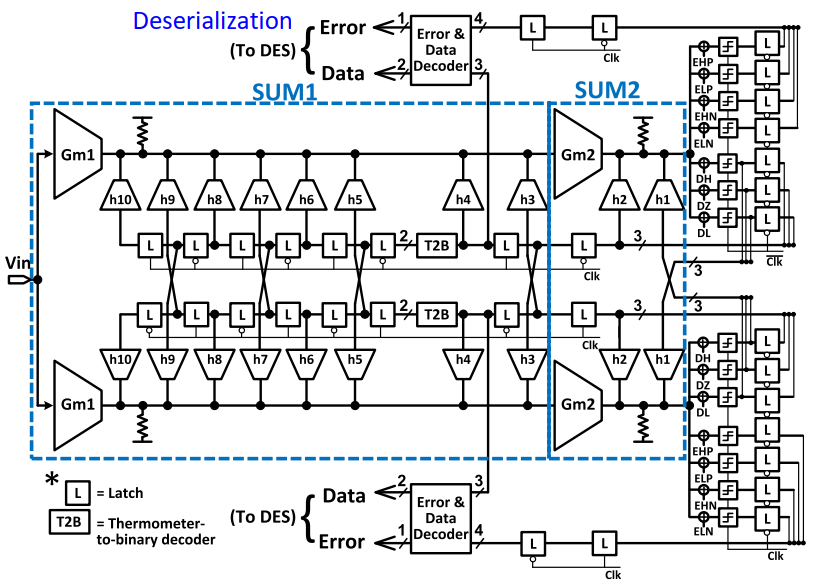
\includegraphics[width=\textwidth]{img/DFE_img/DFE_img_43.png}
        \par\vspace{3pt} % Adds a small vertical space between image and label
        \centerline{(a)} % Centers the label (a) below the image
    \end{minipage}
    \hfill % Horizontal fill space between the two images
    % --- Right Image Container (b) ---
    \begin{minipage}[b]{0.48\textwidth}
        \centering
        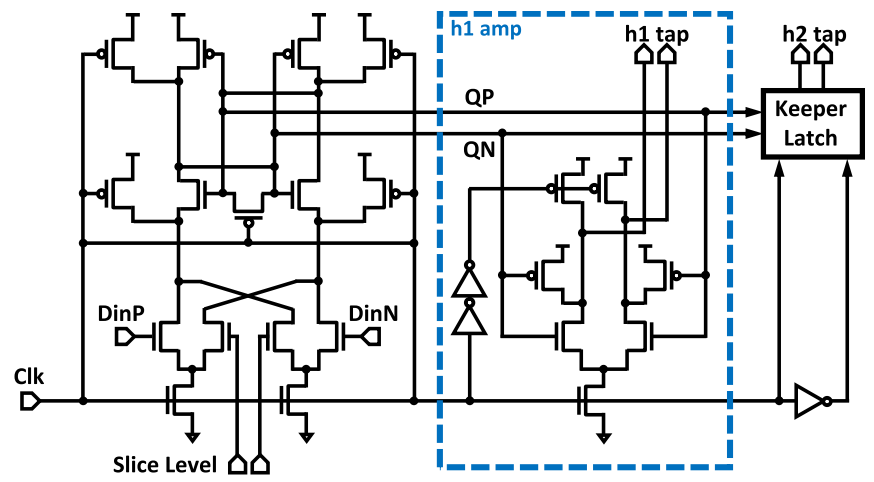
\includegraphics[width=\textwidth]{img/DFE_img/DFE_img_44.png}
        \par\vspace{3pt} % Adds a small vertical space between image and label
        \centerline{(b)} % Centers the label (b) below the image
    \end{minipage}
    
    \vspace{0.5em} % Adds space before the main caption
    \caption{(a) Proposed DFE Architecture (b) Proposed Latch}
    \label{fig:dfe_proposed_1x2} % Good practice to add a label for cross-referencing
\end{figure}

Using Strong-Arm (SA) followed by inverter amplifier. When CLK=0, both outputs of the h1 outputs are pre-charged to supply. This helps maintaining the tail node of the h1 CML tap cell and speeds up h1 settling. When CLK=1, sampling phase occurs in SA causing dip in the common mode voltage. The delay by 2 inverters in the inverter amplifier prevents dip in the output common mode voltage of SA affecting settling time of h1 tap output. h1 tap is taken directly after Master latch.

\begin{figure}[h]
    \centering
    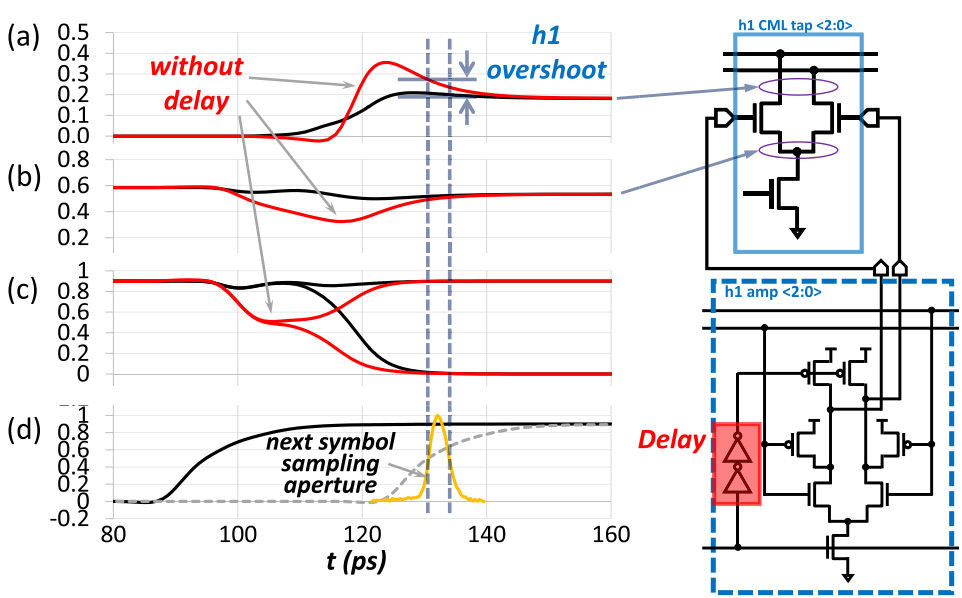
\includegraphics[width=0.55\textwidth]{img/DFE_img/DFE_img_45.png}
    \caption{Delayed pre-charge release of slicer h1 amp. (a) h1 tap current, (b) h1 CML tap tail node, (c) h1 amp output, and (d) slicer sampling clock edges for current (solid line) and the next (dashed line) symbols. Y-axes are in the unit of volts, except (a) which is in mA.}
\end{figure}

\begin{table}[h]
    \centering
    \begin{tabular}{|l|l|}
        \hline
        \textbf{Reference} & \textbf{This Work} \\
        \hline
        Technology & CMOS 16 nm FinFET \\
        \hline
        Modulation & PAM4 \\
        \hline
        Clocking & Half rate \\
        \hline
        Architecture & 10 Taps DFE \\
        \hline
        Supply (V) & 1.2 (analog), 0.9 (digital) \\
        \hline
        Power (mW) & 230 @56Gbps \\
        \hline
        Efficiency (pJ/bit) & 4.107 \\
        \hline
        FoM (pJ/bit/dB) & 0.4107 \\
        \hline
        Data rate (Gbps) & 40-56 \\
        \hline
        Channel Loss (dB) & 10 \\
        \hline
        PRBS Length & 31 \\
        \hline
        BER & $< 10^{-12}$ \\
        \hline
        Area (mm$^2$) & 0.364 \\
        \hline
    \end{tabular}
    \caption{56-Gb/s PAM-4 DFE Specifications}
\end{table}

\newpage
\subsection{Energy Efficient Integrated Summer and Latch-Based DFE (ISL) With Reduced Tap Loading (Nijwm Wary et al., JSSC 2024)}
As shown in Figure \ref{halfrate_proposed} this work proposes merging the summer and the latch into a single cell to make the summer node works in parallel with Latch to relax the timing constrain of first loop. The need of the additional transconductance cell is eliminated by combining the summer and the latch (reducing power consumption). Input of first tap is taken directly after Latch not after SR Latch reducing the loop delay. The proposed half-rate DFE receiver with two taps has been implemented and fabricated in 65 nm CMOS technology. It has been measured at a data rate of 4 Gb/s for a FR4 channel having a loss of 18 dB at Nyquist frequency. The total power consumption of the receiver is 0.938 mW with an energy efficiency of 0.23 pJ/b for a BER < 10-12. The core occupies an area of 993.7 $\mu m^2$.

\begin{figure}[h]
    \centering
    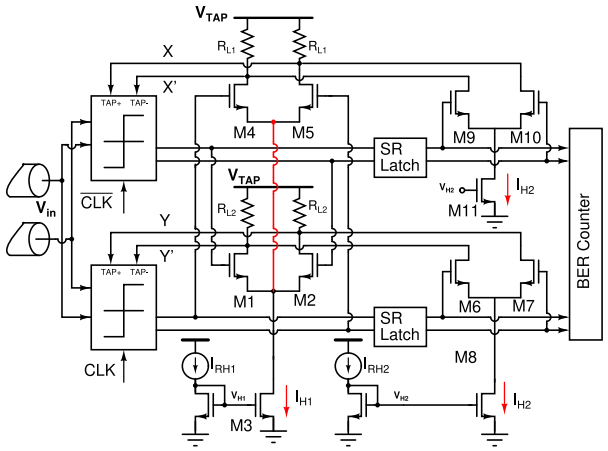
\includegraphics[width=0.5\textwidth]{img/DFE_img/DFE_img_46.png}
    \caption{Proposed Half-Rate DFE}
    \label{halfrate_proposed}
\end{figure}

As shown in Fig \ref{fig:summer_latch_timing}, the difference between conventional and proposed ISL is moving away summer node from sensitive node to less sensitive one which reduces the delay. The other advantage of the proposed DFE is that the power consumption of the first stage of the DTL does not increase with increase in number of taps as the node capacitance at A and B remain unchanged with increase in the number of taps.

fix this too
\begin{figure}[h]
    \centering
    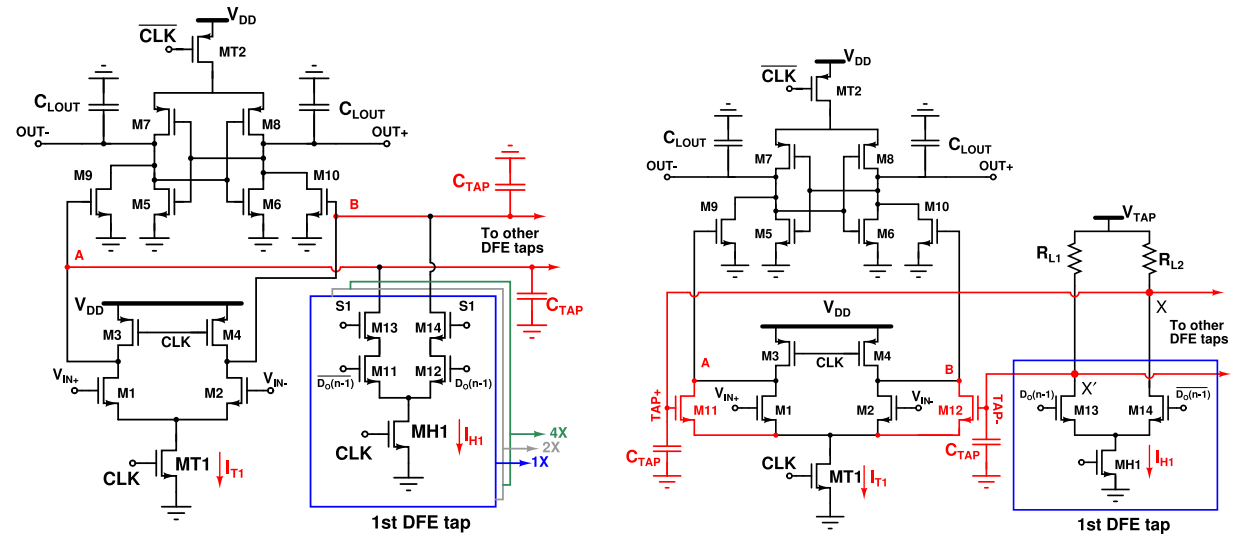
\includegraphics[width=\textwidth]{img/DFE_img/DFE_img_47.png}
    \centerline{(a)\hspace{5cm} (b)}
    \caption{Integrated Summer Latch (a) Conventional (b) proposed}
    \label{fig:summer_latch_timing}
\end{figure}

\begin{figure}[h]
    \centering
    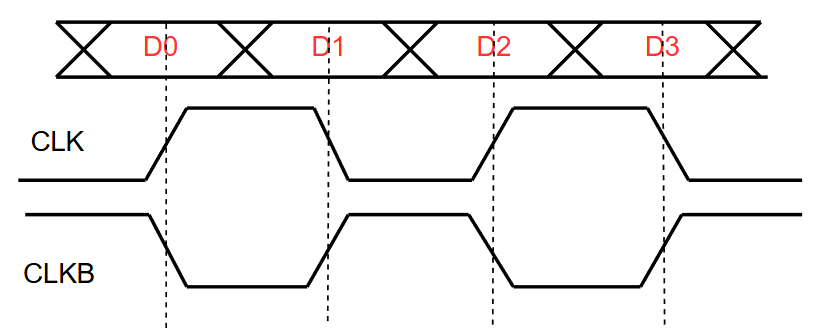
\includegraphics[width=0.3\textwidth]{img/DFE_img/DFE_img_48.png}
    \caption{Timing Diagram}
    \label{fig:timing diagram}
\end{figure}

\begin{figure}[h]
    \centering
    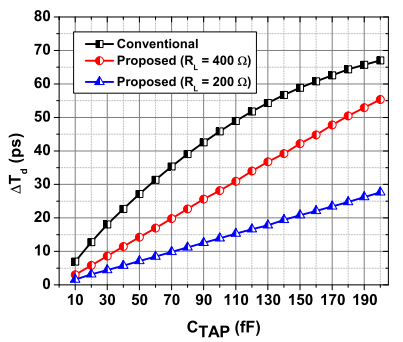
\includegraphics[width=0.35\textwidth]{img/DFE_img/DFE_img_49.png}
    \hfill
    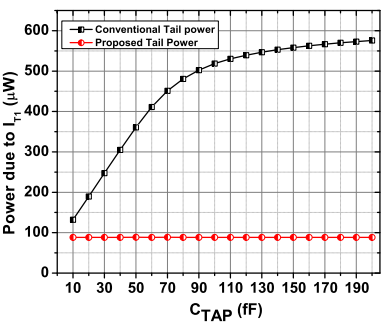
\includegraphics[width=0.35\textwidth]{img/DFE_img/DFE_img_50.png}
    \centerline{(a)\hspace{7cm} (b)}
    \caption{Comparison of variation of delay and power with $C_{TAP}$. (a) Change in delay $\Delta T_d$ (b) Power due to $I_{T1}$.}
\end{figure}

\begin{table}[h]
    \centering
    \begin{tabular}{|l|l|}
        \hline
        \textbf{Reference} & \textbf{This Work} \\
        \hline
        Technology & 65 nm \\
        \hline
        Modulation & NRZ \\
        \hline
        Clocking & Half rate \\
        \hline
        Architecture & 2 Taps DFE \\
        \hline
        Supply (V) & 1.2 \\
        \hline
        Efficiency (pJ/bit) & 0.23 \\
        \hline
        FoM (pJ/bit/dB) & 0.013 \\
        \hline
        Data rate (Gbps) & 4 \\
        \hline
        Channel Loss (dB) & 18 \\
        \hline
        PRBS Length & 15 \\
        \hline
        BER & $< 10^{-12}$ \\
        \hline
        Area ($\mu m^2$) & 993.65 \\
        \hline
    \end{tabular}
    \caption{ISL DFE Specifications}
\end{table}

\subsection{A 60-Gb/s PAM4 Wireline Receiver With 2-Tap DFE Employing Track-and-Regenerate Slicer (Azita Emami et al., JSSC 2020)}
\textbf{CMOS Track and Regenerate Slicer:}

Instead of the differential output signal grows from approximately zero, it begins with a higher level. The Latch will operate for the whole clock period (like CML) which includes \textbf{Track} phase and \textbf{Regeneration} phase. It consists of 3 stages: 2 preamp and 1 regeneration. M15 and M16 are kept always on with weak currents to prevent cross coupled from being completely off (small static current).

\begin{figure}[H]
    \centering
    % --- Top Row: Image (a) ---
    \begin{minipage}[b]{0.5\textwidth}
        \centering
        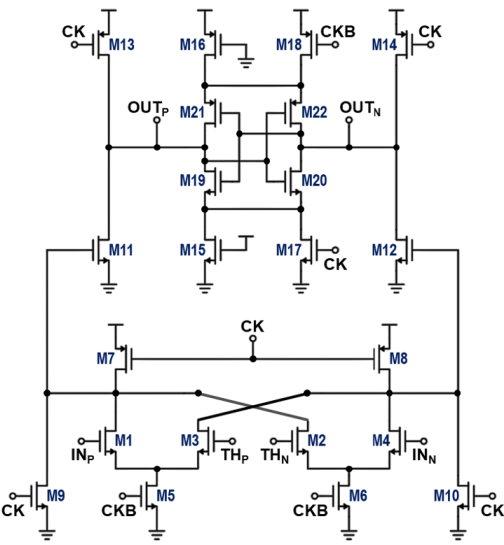
\includegraphics[width=.7\textwidth]{img/DFE_img/DFE_img_51.png}
        \par\vspace{3pt}
        \centerline{(a) Proposed Latch}
    \end{minipage}
    
    \vspace{1em} % Space between the rows

    % --- Bottom Row: Images (b) and (c) ---
    \begin{minipage}[b]{0.48\textwidth}
        \centering
        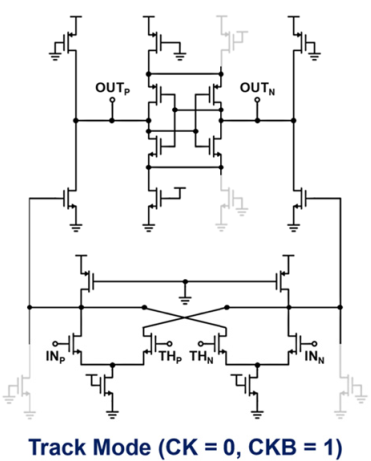
\includegraphics[width=.65\textwidth]{img/DFE_img/DFE_img_52.png}
        \par\vspace{3pt}
        \centerline{(b) Track Mode}
    \end{minipage}
    \hfill
    \begin{minipage}[b]{0.48\textwidth}
        \centering
        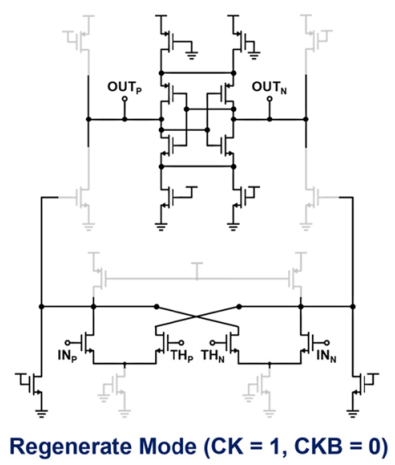
\includegraphics[width=.65\textwidth]{img/DFE_img/DFE_img_53.png}
        \par\vspace{3pt}
        \centerline{(c) Regenerate Mode}
    \end{minipage}

    \vspace{0.5em}
    \caption{Operation of the proposed latch: (a) Circuit Schematic, (b) Track Mode equivalent, and (c) Regenerate Mode equivalent.}
    \label{fig:latch_operation}
\end{figure}


\textbf{Advantages:}
\begin{itemize}
    \item Huge difference in diff input sensitivity at high baud rate due to tracking phase in proposed CMOS.
    \item Less sensitive to VDD variations.
\end{itemize}

\begin{table}[h]
    \centering
    \begin{tabular}{|l|l|l|}
        \hline
        \textbf{VDD} & \textbf{Proposed Slicer $T_{cq}$} & \textbf{Strong-Arm $T_{cq}$} \\
        \hline
        900mV & 15.34 ps & 30.96 ps \\
        \hline
        850mV & 17.7 ps & Didn't reach VDD/2 \\
        \hline
    \end{tabular}
    \caption{Comparison of Proposed Slicer vs Strong-Arm}
\end{table}

As shown in Fig \ref{timing first tap}, since the operations take place concurrently, $T_{dh1}\ and\ T_{settle}$ are additional delay with respect to $T_{cq}$ during which the DFE tap currents and the summer have already started to settle toward their steady states.

\begin{figure}[h]
    \centering
    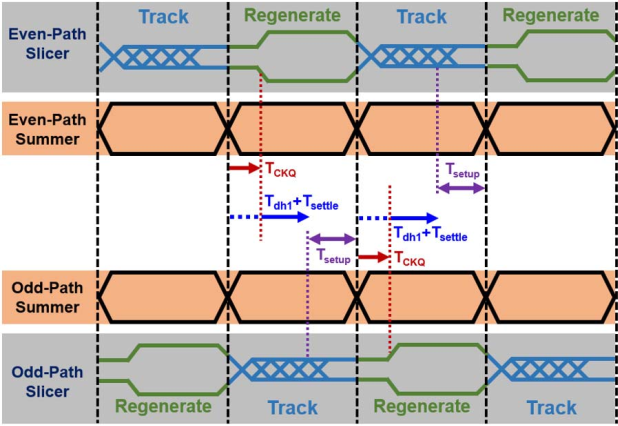
\includegraphics[width=0.4\textwidth]{img/DFE_img/DFE_img_54.png}
    \caption{Timing diagram for the first tap DFE in a half-rate design, and the simulated numbers for the timing constraints at 30 GBaud/s}
    \label{timing first tap}
\end{figure}

\begin{table}[h]
    \centering
    \begin{tabular}{|l|l|l|l|}
        \hline
        Weak Symbols & $T_{cq}$ & $T_{dh1} + T_{settle}$ & $T_{setup}$ \\
        \hline
        & $\sim$ 16ps & 3.65 ps (85\% settling) & 9.9 ps \\
        \cline{3-3}
        & & 5.51 ps (90\% settling) & \\
        \cline{3-3}
        & & 8.36 ps (95\% settling) & \\
        \hline
    \end{tabular}
    \caption{Timing Constraints for Weak Symbols}
\end{table}

\begin{figure}[h]
    \centering
    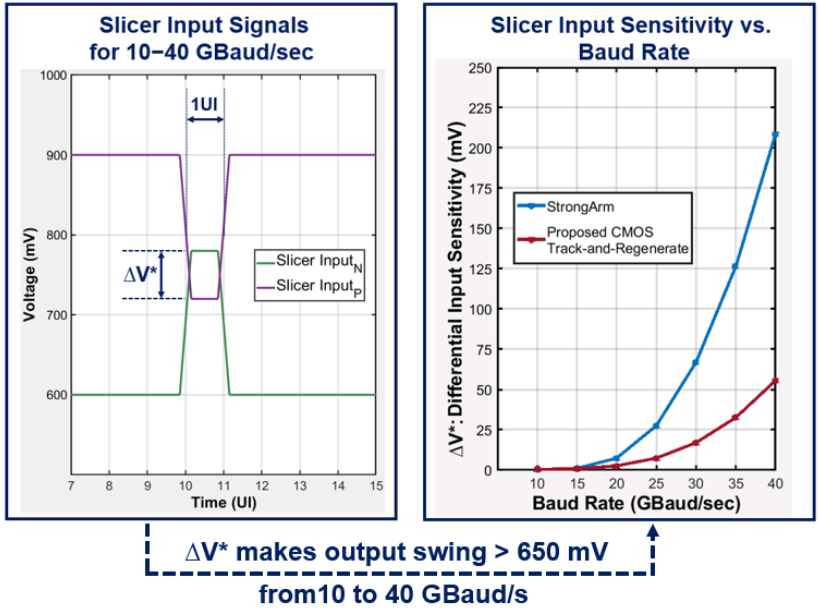
\includegraphics[width=0.55\textwidth]{img/DFE_img/DFE_img_55.png}
    \caption{Measured Differential Input Sensitivity at worst case}
\end{figure}

\begin{table}[h]
    \centering
    \begin{tabular}{|l|l|l|}
        \hline
        \textbf{Reference} & \textbf{Proposed Slicer} & \textbf{Strong Arm} \\
        \hline
        $T_{cq}$ & $\sim < 16ps$ & $\sim < 31ps$ \\
        \hline
        Input-referred noise ($mV_{rms}$) & 1.69 & 3.37 \\
        \hline
        Power consumption (mW) & 1.7 & 0.43 \\
        \hline
        Differential Offset Standard Deviation (mV) & 18.3 & 20.9 \\
        \hline
        Required Clock phase & 2 & 1 \\
        \hline
    \end{tabular}
    \caption{Performance Comparison: Proposed Slicer vs Strong Arm}
\end{table}

\newpage
\textbf{Common Mode Restoration for Summer node:}

Since input common mode voltage variations affect the delay of the Latch it is important to work at optimum common mode voltage to achieve best delay. In this paper it has proposed a circuit to restore common mode as shown in Fig \ref{fig:cmr_circuit}

\begin{figure}[htbp]
    \centering
    % --- Left Subfigure ---
    \begin{subfigure}[b]{0.48\textwidth}
        \centering
        % Width is relative to the subfigure container, not the page
        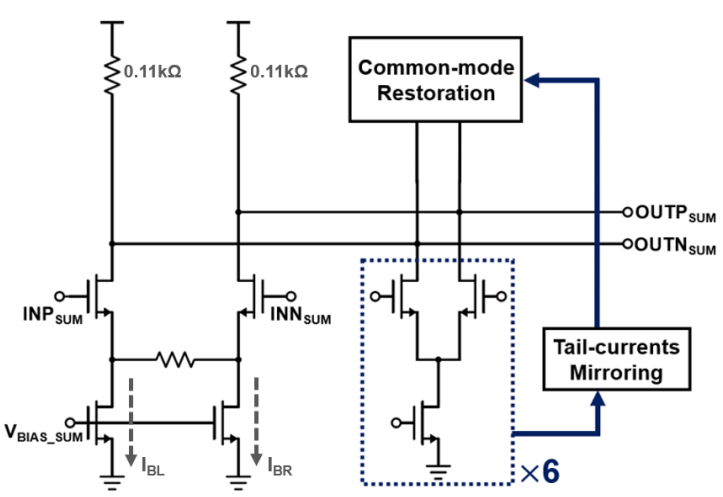
\includegraphics[width=.8\textwidth]{img/DFE_img/DFE_img_56.png}
        \caption{Architecture of the summer for 2-tap DFE}
        \label{fig:summer}
    \end{subfigure}
    \hfill % Adds flexible space between the images
    % --- Right Subfigure ---
    \begin{subfigure}[b]{0.48\textwidth}
        \centering
        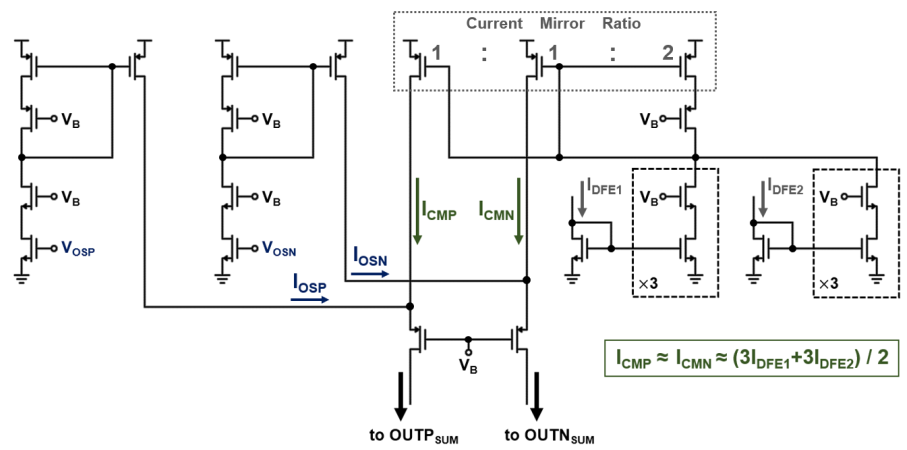
\includegraphics[width=.8\textwidth]{img/DFE_img/DFE_img_57.png}
        \caption{Schematic of the common-mode restoration circuits}
        \label{fig:cmr_circuit}
    \end{subfigure}
    
    \caption{Implementation details of the DFE Summer and Common-Mode Restoration circuits.}
    \label{fig:dfe_implementation}
\end{figure}

\begin{figure}
    \centering
    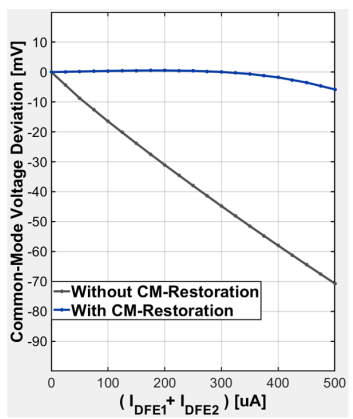
\includegraphics[width=0.4\textwidth]{img/DFE_img/DFE_img_58.png}
    \caption{Simulated performance of the common-mode restoration circuits, showing the deviation from the target common mode with and without the common-mode restoration circuits.}
\end{figure}


\begin{table}[h]
    \centering
    \renewcommand{\arraystretch}{1} % Slightly more space
    \begin{tabular}{ll} % No vertical bars |
        \toprule
        \textbf{Parameter} & \textbf{Value} \\ % I renamed the headers for clarity
        \midrule
        Technology & 28 nm CMOS \\
        Modulation & PAM4 \\
        Clocking & Half rate \\
        Architecture & 2 Taps DFE \\
        Supply & 0.9 V \\
        Efficiency & 1.1 pJ/bit \\
        FoM & 0.134 pJ/bit/dB \\
        Data rate & 60 Gbps \\
        Channel Loss & 8.2 dB \\
        BER & $< 10^{-12}$ \\
        \bottomrule
    \end{tabular}
    \caption{60-Gb/s PAM4 Receiver Specifications}
\end{table}